\documentclass{article}

% Language setting
% Replace `english' with e.g. `spanish' to change the document language
\usepackage[english]{babel}

% Set page size and margins
% Replace `letterpaper' with `a4paper' for UK/EU standard size
\usepackage[letterpaper,top=2cm,bottom=2cm,left=3cm,right=3cm,marginparwidth=1.75cm]{geometry}

% Useful packages
\usepackage{amsmath}
\usepackage{graphicx}
\usepackage[colorlinks=true, allcolors=blue]{hyperref}
\usepackage{listings}
\usepackage{authblk}

\title{\textbf{Pricing Analysis Platform}}

\usepackage{xcolor}

%New colors defined below
\definecolor{codegreen}{rgb}{0,0.6,0}
\definecolor{codegray}{rgb}{0.5,0.5,0.5}
\definecolor{codepurple}{rgb}{0.58,0,0.82}
\definecolor{backcolour}{rgb}{0.95,0.95,0.92}

%Code listing style named "mystyle"
\lstdefinestyle{mystyle}{
  backgroundcolor=\color{backcolour}, commentstyle=\color{codegreen},
  keywordstyle=\color{purple},
  numberstyle=\tiny\color{codegray},
  stringstyle=\color{codepurple},
  basicstyle=\ttfamily\footnotesize,
  breakatwhitespace=false,         
  breaklines=true,                 
  captionpos=b,                    
  keepspaces=true,                 
  numbers=left,                    
  numbersep=5pt,                  
  showspaces=false,                
  showstringspaces=false,
  showtabs=false,                  
  tabsize=2
}

%"mystyle" code listing set
\lstset{style=mystyle}

\author{Bruno Campos U., Iván Serrano Z., Luis Noguera G., Maximino Navarro M. 
\\ José María Sarmiento Chávez}
\affil[]{Universidad Panamericana 
\\Maestría en Ciencia de Datos}

\begin{document}

\begin{figure}

\includegraphics[width=0.4\linewidth]{Reports/images/up_logo.jpg}
\end{figure}

\maketitle

\section{Resumen Ejecutivo}

En este trabajo se plantea la propuesta de crear una plataforma para \textbf{analizar} y \textbf{predecir} los precios de la canasta básica alimentaria, utilizando datos de "Quién es Quién en los Precios" de la Profeco y herramientas como \textbf{Hadoop}, \textbf{Spark}, \textbf{python} y \textbf{Google Cloud Platform}. El objetivo es mejorar la capacidad de planificación de compras informadas para los consumidores, mediante la generación de modelos predictivos que permitan anticipar las fluctuaciones de precios. Esto no solo proporcionará a los consumidores una herramienta estratégica para la gestión de su presupuesto, sino que también contribuirá a resolver problemas socioeconómicos al brindar información valiosa para la formulación de políticas públicas orientadas a garantizar el acceso a alimentos asequibles y promover el bienestar económico de la población. El uso del \textbf{Big Data} en este contexto no solo permite comprender las tendencias históricas de precios, sino también identificar patrones predictivos que pueden ser utilizados para anticipar las fluctuaciones futuras, ofreciendo así una visión más clara y anticipada de la dinámica de precios en el mercado de alimentos básicos.

\subsection{Introducción}

En México, se han llevado a cabo importantes trabajos con el objetivo de definir una canasta que refleje las necesidades básicas de los mexicanos. Entre ellos, destacan la Canasta Normativa de Satisfactores Esenciales (CNSE), la Canasta Alimentaria propuesta por la Comisión Económica para América Latina y el Caribe (CEPAL) en colaboración con el INEGI, y las canastas Alimentaria y No Alimentaria del CONEVAL.

La CNSE se desarrolló a partir de la Encuesta de Ingresos y Gastos Familiares de 1975 del Centro Nacional de Información y Estadísticas del Trabajo, con el objetivo de reflejar los patrones de consumo frecuentes en la población mexicana, así como cumplir con las normativas y objetivos establecidos por la legislación mexicana.

La Canasta Alimentaria, creada por el CEPAL y el INEGI en 1998, tuvo como propósito reflejar las necesidades nutricionales de la población mexicana. Esta iniciativa formó parte de un esfuerzo más amplio para homogeneizar la metodología de medición de la pobreza en América Latina.

Posteriormente, en 2004, la Ley General de Desarrollo Social (LGDS) estableció la creación del CONEVAL con el fin de normar y coordinar la evaluación de políticas y programas de desarrollo social, así como definir, identificar y medir la pobreza. En 2010, el CONEVAL publicó una canasta alimentaria para los ámbitos rural y urbano, adaptando la metodología desarrollada por la CEPAL y el INEGI, así como una canasta no alimentaria basada en la propuesta metodológica de Hernández Laos. Estas canastas fueron diseñadas para medir la pobreza multidimensional, una de las funciones principales del CONEVAL.

La Procuraduría Federal del Consumidor (Profeco) recopila los precios de 200 000 productos específicos en aproximadamente 1 500 establecimientos comerciales, productos que representan alrededor de 3 600 marcas, variedades y presentaciones. Estos precios son presentados a través de un programa denominado “Canasta Inteligente”, que permite al usuario crear su propia canasta en función de sus necesidades, a fin de darle a conocer los precios mínimos y promedio, así como el mejor lugar de compra. Asimismo, se presentan catálogos que asocian un conjunto de productos con base en la Canasta Básica y la información de gasto de la Encuesta Nacional de Ingresos y Gastos de los Hogares que realiza el INEGI. 

\section{Visión general del desarrollo}

La Profeco realiza un seguimiento quicenal de los precios de un listado de productos básicos y de alto consumo para la alimentación de la población mexicana a través de su portal de \href{https://www.profeco.gob.mx/precios/canasta/qqpc.php}{Quién es Quién en los precios (QQP)} (ver figura 1). Poder contar con estos datos es indipensable para analizar la variación en los precios de estos productos y saber cómo dichas variaciones de precios podrían impactar a los consumidores con menos recursos, esta lógica es la que se usa para generar el índice Nacional de Precios al Consumidor (INPC) el cuál es usa para medir la inflación.

\begin{figure}[h]
\centering
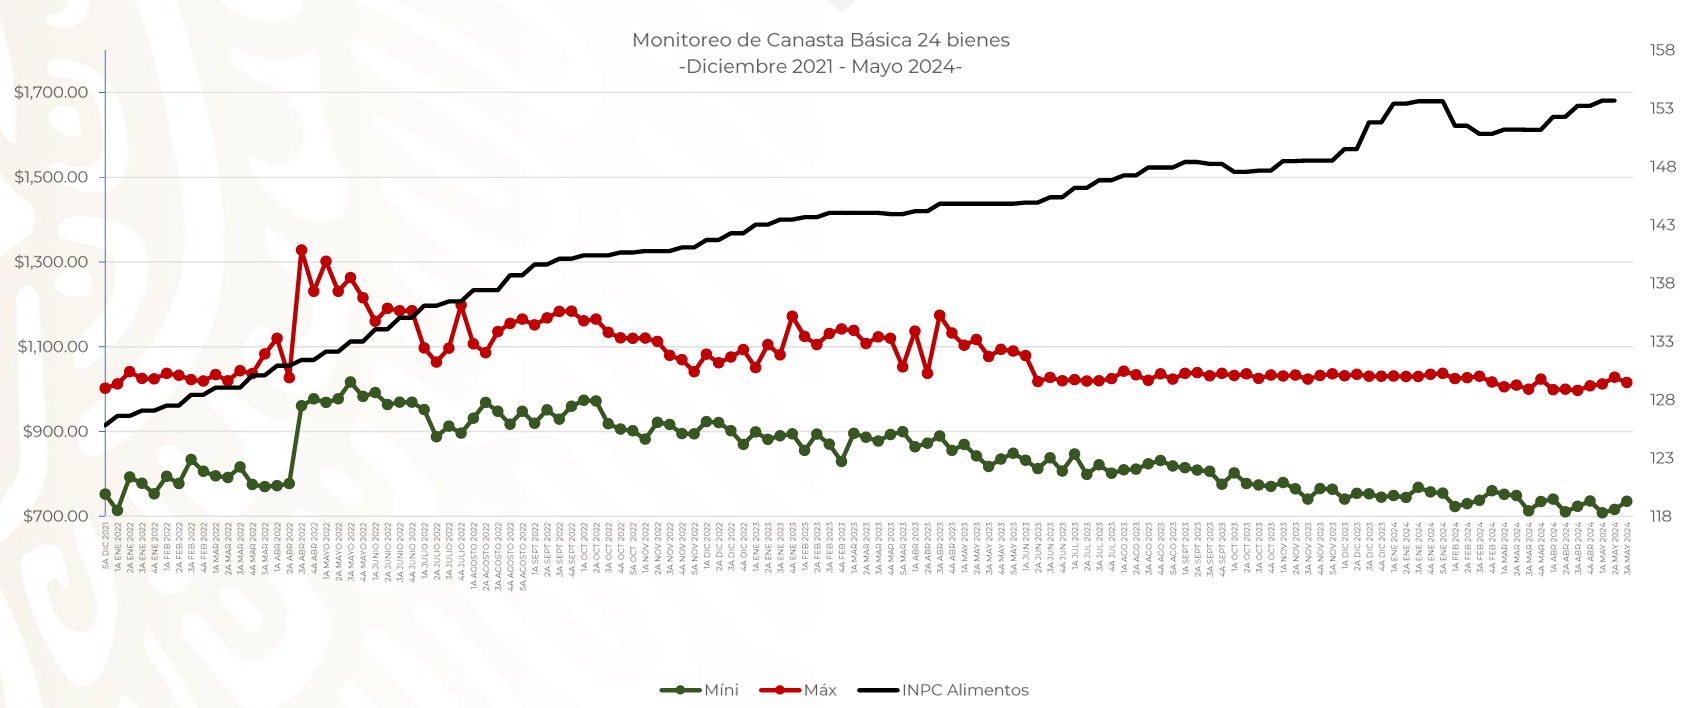
\includegraphics[width=0.8\linewidth]{Reports/images/Tendencia.png}
\caption{\label{fig:Canasta}Seguimiento de canasta básica por QQP}
\end{figure}

\subsection{Solución Actual / visión general}
La Profeco, además de dar un seguimiento quicenal a los precios de los productos, genera un reporte semanal con el Top 5 de los precios máximos y mínimos de una canasta de 24 alimentos (ver figura 2) que fueron tomandos de la canasta alimentaria definida por el CONEVAL y muestra dicho análisis por las distintas regiones de México (las regiones definidas por El Banco de México (BANXICO) en su Reporte sobre las economías regionales, julio-septiembre 2021). 

\begin{figure}[h]
\centering
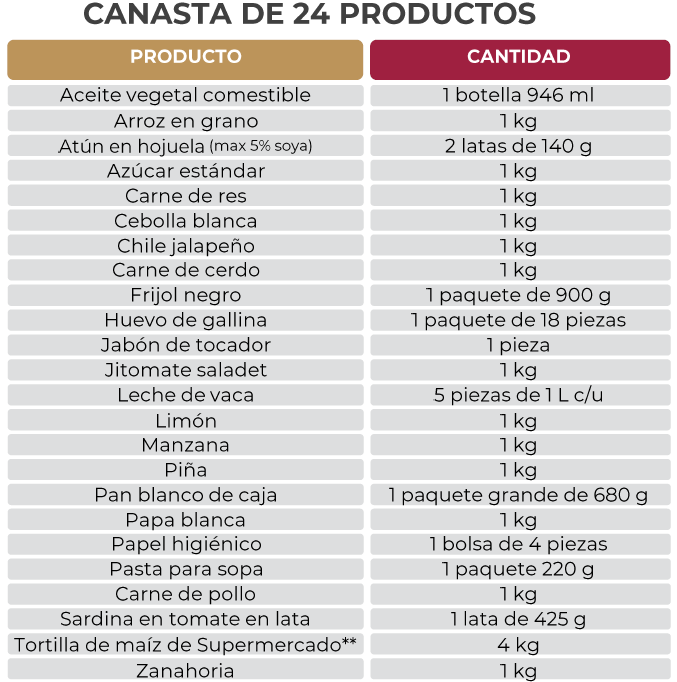
\includegraphics[width=0.7\linewidth]{Reports/images/Canasta.png}
\caption{\label{fig:Architecture}Canasta Básica de 24 productos(basados en la Cantasta definida por el CONEVAL}
\end{figure}

\newpage 
El reporte de \textbf{QQP} muestra dicha información con el detalle del establecimiento, la entidad, municipio, domicilio y el precio de referencia (ver figura 3) para que los consumidores puedan estar realizar comparaciones y realizar sus comprar de manera más informada.

\begin{figure}[h]
\centering
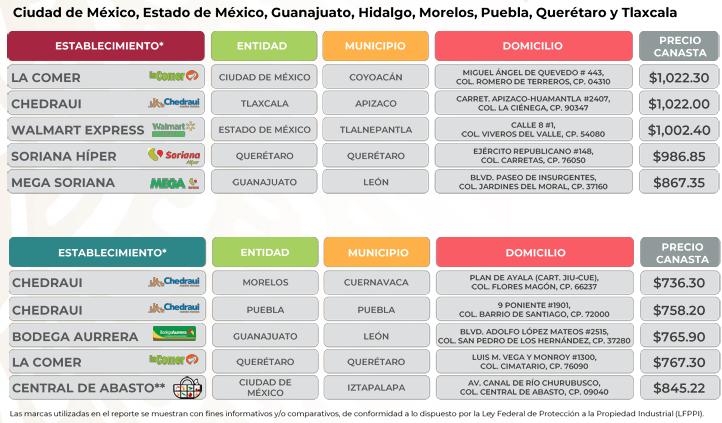
\includegraphics[width=0.9\linewidth]{images/Top 5.png}
\caption{\label{fig:Canasta}Top 5 de los precios mínimos y máximos en la región centro del país}
\end{figure}

\subsection{Propósito, uso y alcance de la herramienta}

\section{Revisión y uso de datos}

Hola crayola Hola hola

\subsection{Orígenes y control de datos}

El programa Quién es Quién en los Precios (QQP) recopila y difunde información sobre precios de productos domésticos de consumo habitual, como alimentos, bebidas, productos de cuidado personal, artículos para el hogar, medicamentos, electrodomésticos y artículos de temporada. Esta información tiene como objetivo ayudarle a tomar decisiones de compra informadas mediante la comparación de precios.

Los precios se recogen visitando una muestra de los principales establecimientos de cada una de las ciudades participantes en el programa durante los cinco días hábiles de la semana.

Los precios mostrados incluyen la fecha en que fueron tomados; sin embargo, están sujetos a cambios ya que algunos establecimientos pueden variar sus precios más de una vez al día. Por tanto, deben considerarse precios de referencia.

\subsubsection{Extracción, Transformación y Carga de datos}

Para la extracción de los datos se hizo mediante un scrapper desarrollado en python usando las siguientes bibliotecas:
\begin{lstlisting}[language=Python]
    from lxml import html
    import requests
    import re
    import os
\end{lstlisting}

Se entra a la página de QQP \textit{https://www.profeco.gob.mx/precios/canasta/qqpc.php} y se hace todo el procedimiento de exploración y extracción de distintas partes de la página para encontrar las secciones de HTML que contienen los archivos csv. Después se crea un proceso que extraerá uno por uno los archivos que fueron cargados de forma quicenal y se guardan en carpetas con el nombre del mes, año y la quincena a la que corresponde en archivos rar. 

\begin{lstlisting}[language=Python, caption={python version}]

page=requests.get('https://datos.profeco.gob.mx/datos_abiertos/qqp.php')
tree = html.fromstring(page.content)

links = tree.xpath('/html/body/main/div/div//@href')

names = tree.xpath('/html/body/main/div/div//a/text()')

clean_year = ['QQP_'+re.findall(r'\d+',s)[0] for s in names]

pages = dict(zip(clean_year,links))

def create_folder_if_not_exists(folder_name):
    if not os.path.exists(folder_name):
        os.makedirs(folder_name)
        print(f"The folder '{folder_name}' has been created.")
    else:
        print(f"The folder '{folder_name}' already exists.")

for year in pages:
    print(year, "->", pages[year])

home = 'https://datos.profeco.gob.mx/datos_abiertos/'

def download_files(home, json_pages):
    for year in json_pages:
        url = home + json_pages[year]
        print('Trying to download {} -> {}'.format(url, year))
        try:
            response = requests.get(url)
            if response.status_code == 200:
                create_folder_if_not_exists("files/{year}".format(year = year))
                with open("files/{year}/{year}.rar".format(year = year), "wb") as file:
                    file.write(response.content)
                    print("File downloaded successfully!")
            else:
                print("Failed to download the file.")
        except Exception as e:
                print(f"Failed to open the menu. \n Error: {e}")
download_files(home, pages)
\end{lstlisting}

Posteriormente se ejecuta el script para la descompresión de los archivos rar.

\begin{lstlisting}[language=bash,caption={bash version}]
#!/bin/bash

# Instalar rar y unrar si no estan instalados
sudo apt update && sudo apt upgrade -y
sudo apt install -y rar unrar

# Obtener el directorio base desde el argumento de la linea de comandos
base_dir="$1"

# Verificar si se proporciona un directorio base
if [ -z "$base_dir" ]; then
  echo "Uso: $0 <directorio>"
  exit 1
fi

# Verificar si el directorio base existe
if [ ! -d "$base_dir" ]; then
  echo "El directorio base '$base_dir' no existe."
  exit 1
fi

# Listar todos los directorios en el directorio base
for dir in "$base_dir"/*; do
  if [ -d "$dir" ]; then
    # Extraer el nombre del directorio
    dir_name=$(basename "$dir")
    
    # Definir la ruta del archivo .rar
    rar_file="$dir/$dir_name.rar"
    
    # Definir el directorio de salida csv
    csv_dir="$dir/csv"
    
    # Crear el directorio csv si no existe
    mkdir -p "$csv_dir"
    
    # Extraer el archivo .rar en el directorio csv
    unrar e "$rar_file" "$csv_dir"
  fi
done
\end{lstlisting}

\newpage
Para más detalle de cómo realizar la extracción de los datos, remitirse a la sección correspondiente de \textit{Data Extraction and Analysis Platform} \href{https://github.com/Anonymate054/MCD-BigData/tree/main/Scrapper}{MCD-BigData/tree/main/Scrapper} (ver figura 4), dentro del Github del proyecto y seleccionar el archivo \textit{Scrapper.ipynb} que se encuentra dentro de la siguiente ruta: \textit{Scrapper/notebooks/Python-classic/}.


\begin{figure}[h]
\centering
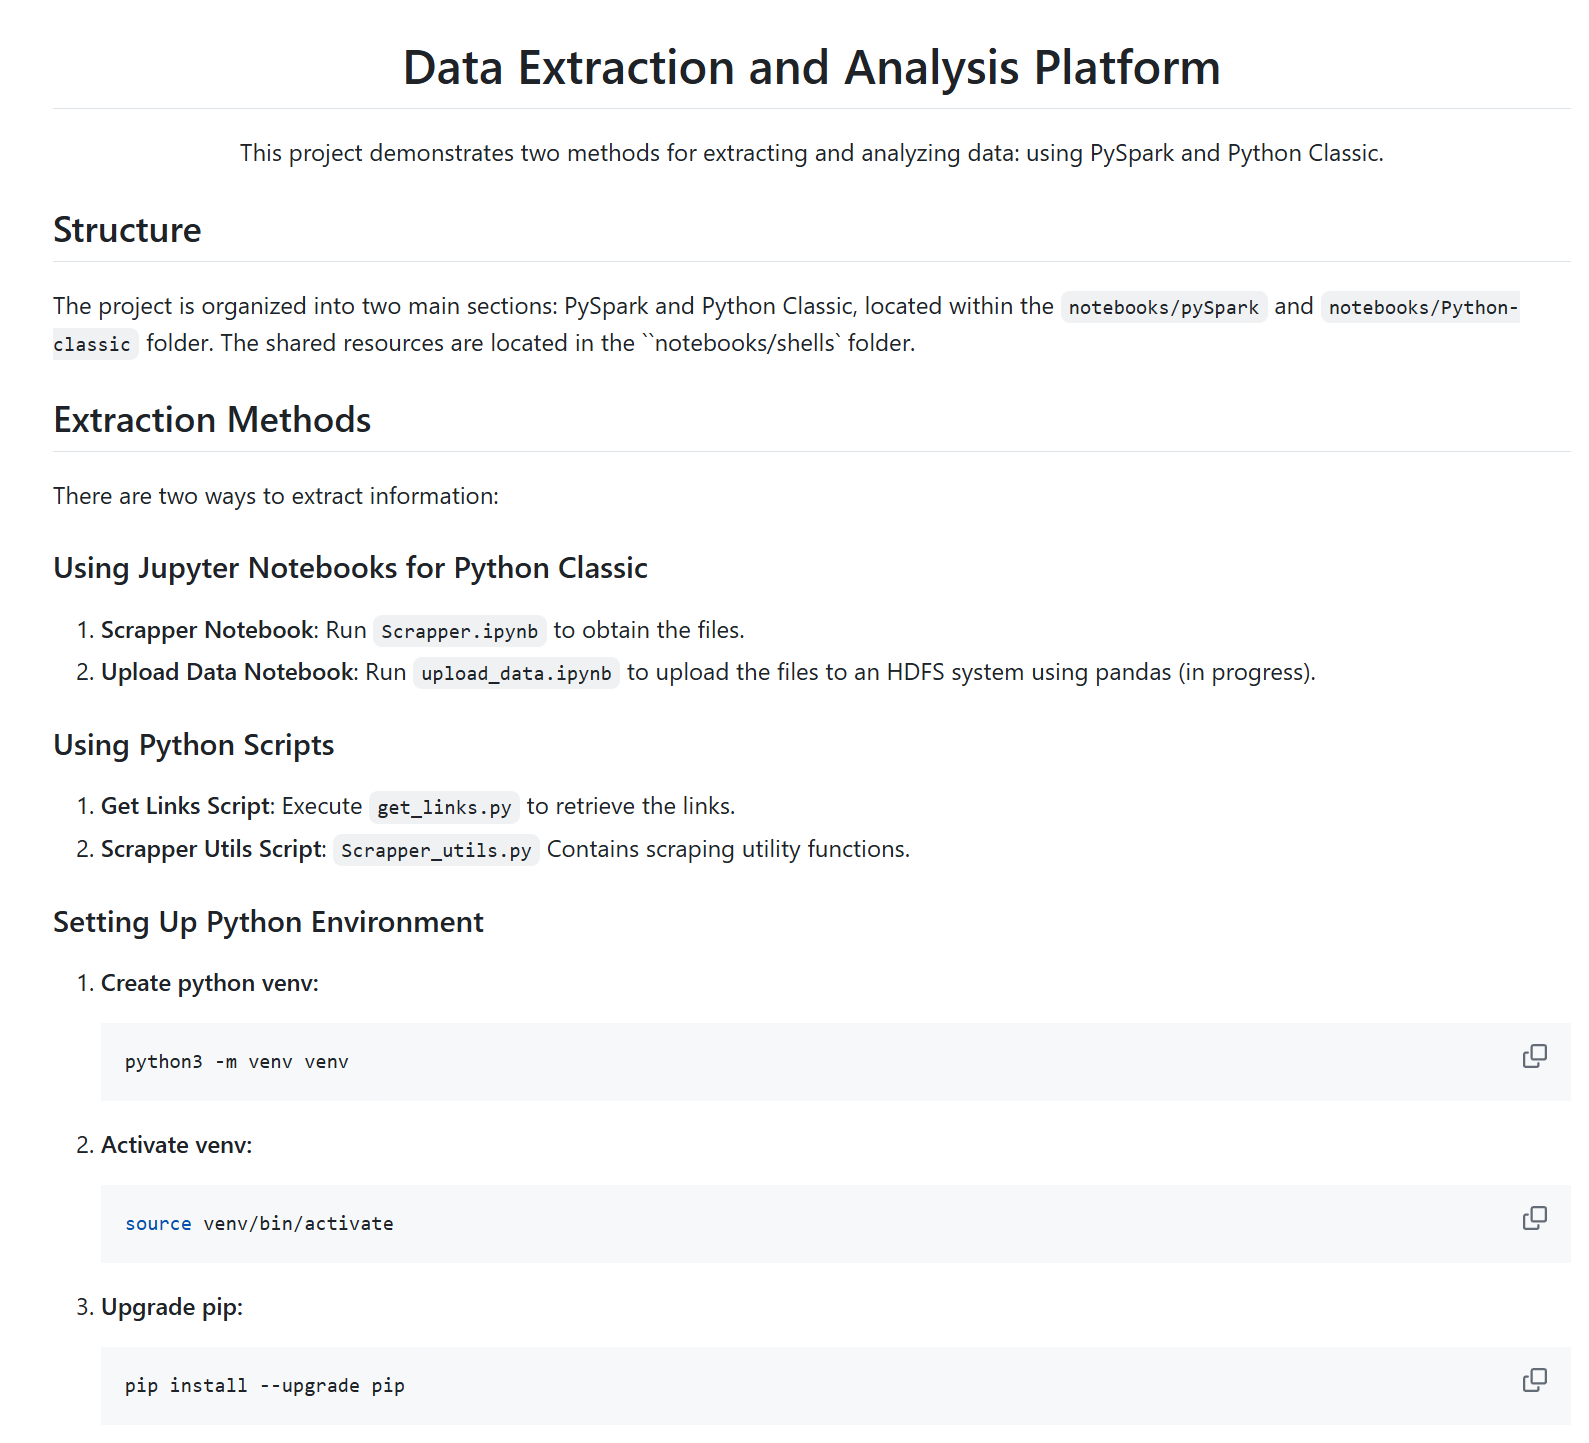
\includegraphics[width=0.7\linewidth]{Reports/images/Extraction.png}
\caption{\label{fig:Extracción}Instrucciones para crear el entorno virtual y extraer los datos de Quién es Quién en los Precios}
\end{figure}


Dentro del directorio de \textit{Python classic} podrán encontrar los siguientes archivo adicionales:

\begin{figure}[h]
\centering
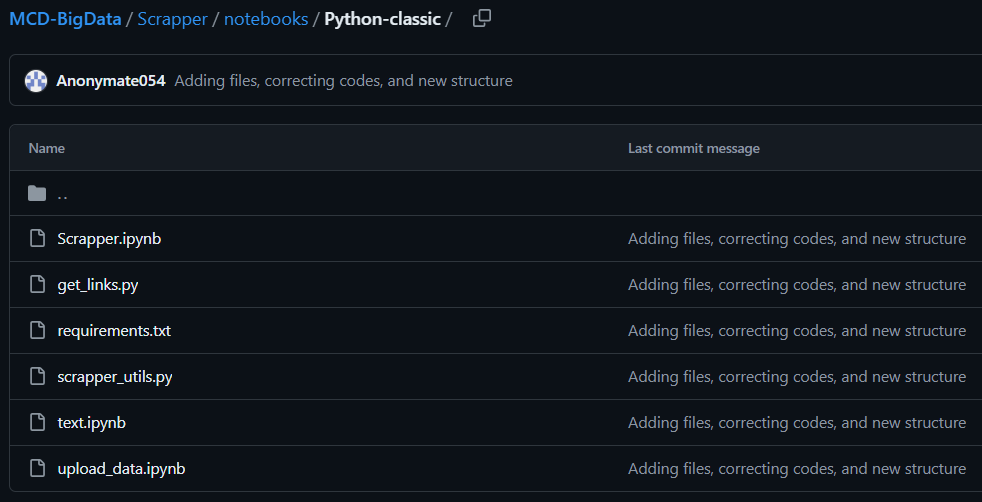
\includegraphics[width=0.7\linewidth]{Reports/images/files.png}
\caption{\label{fig:files}Archivos adicionales}
\end{figure}

\newpage
Una vez extraída toda la información de la página, se hace un compendio de ellas y se mandan al HDFS dentro del mismo notebook que se usó para extraer la información. 

\begin{lstlisting}[language=Python]
### Import libraries
from pyspark.sql import SparkSession
from pyspark.sql.functions import lit
from datetime import datetime
from pyspark.sql.types import StructType, StructField, IntegerType, StringType, DecimalType

from IPython.core.display import HTML
display(HTML("<style>pre { white-space: pre !important; }</style>"))

warehouse_location = '/files'

### Create spark session
spark = SparkSession \
    .builder \
    .appName("App de Spark para QQP") \
    .config("spark.sql.warehouse.dir", warehouse_location) \
    .enableHiveSupport() \
    .getOrCreate()

### Print spark info
spark

### List files on hdfs
!hdfs dfs -ls /user/QQP | head -n 6

%%time
!hdfs dfs -count /user/QQP

schema = StructType([
    StructField("PRODUCTO", StringType(), True),
    StructField("PRESENTACIÓN", StringType(), True),
    StructField("MARCA", StringType(), True),
    StructField("CATEGORÍA", StringType(), True),
    StructField("CATÁLOGO", StringType(), True),
    StructField("PRECIO", DecimalType(18, 2), True),
    StructField("FECHAREGISTRO", StringType(), True),
    StructField("CADENACOMERCIAL", StringType(), True),
    StructField("GIRO", StringType(), True),
    StructField("NOMBRECOMERCIAL", StringType(), True),
    StructField("DIRECCIÓN", StringType(), True),
    StructField("ESTADO", StringType(), True),
    StructField("MUNICIPIO", StringType(), True),
    StructField("LATITUD", DecimalType(18, 6), True),
    StructField("LONGITUD", DecimalType(18, 6), True)
])

df = spark.read.csv('/user/QQP/', sep=',', header=False, schema=schema)

# Get the list of input files
file_list = df.inputFiles()
print("Number of input files: ", len(file_list))

%%time
df.count()

%%time
df.count()

### Load data into QQP table
df.write.mode('overwrite').saveAsTable('QQP')

### Close spark session
spark.stop()

\end{lstlisting}

\newpage
\subsubsection{Arquitectura de solución completa}
\begin{figure}[h]
\centering
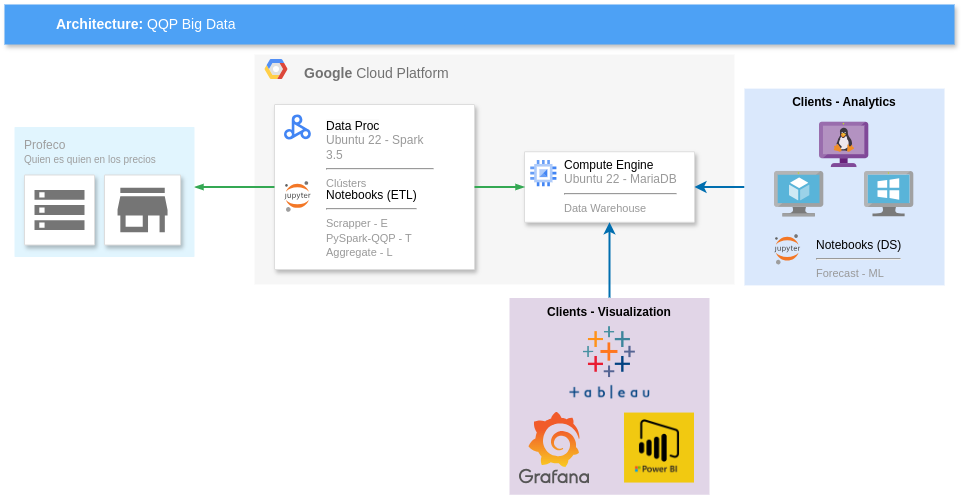
\includegraphics[width=0.9\linewidth]{images/Architecture_QQP_BD.png}
\caption{\label{fig:Architecture}This frog was uploaded via the file-tree menu.}
\end{figure}

\subsection{Limpieza y tratamiento de datos}

First you have to upload the image file from your computer using the upload link in the file-tree menu. Then use the includegraphics command to include it in your document. Use the figure environment and the caption command to add a number and a caption to your figure. See the code for Figure \ref{fig:frog} in this section for an example.

{including images on Overleaf}.

\subsection{Limitaciones de los datos}

Use the table and tabular environments for basic tables --- see Table~\ref{tab:widgets}, for example. For more information, please see this help article on \href{https://www.overleaf.com/learn/latex/tables}{tables}. 

\section{Proceso de desarrollo}

Use the table and tabular environments for basic tables --- see Table~\ref{tab:widgets}, for example. For more information, please see this help article on \href{https://www.overleaf.com/learn/latex/tables}{tables}. 

\subsection{Metodología}

La metodología CRISP-DM (Cross Industry Standard Process for Data Mining) es un modelo estándar ampliamente utilizado en la minería de datos y en el campo de la ciencia de datos. Proporciona un marco estructurado para planificar y ejecutar proyectos de minería de datos, y se compone de seis fases principales:

\begin{enumerate}
\item \textbf{Comprensión del Negocio (Business Understanding):}

\begin{itemize}
\item Objetivo: Entender los objetivos y requisitos del proyecto desde una perspectiva de negocio.
\item Tareas: Definir los objetivos del negocio, evaluar la situación actual, definir los objetivos de minería de datos y producir un plan de proyecto.
\end{itemize}

\item \textbf{Comprensión de los Datos (Data Understanding):}

\begin{itemize}
\item Objetivo: Familiarizarse con los datos y evaluar su calidad.
\item Tareas: Recolectar datos iniciales, describir los datos, explorar los datos y verificar la calidad de los datos.
\end{itemize}

\item \textbf{Preparación de los Datos (Data Preparation):}

\begin{itemize}
\item Objetivo: Preparar los datos en una forma que pueda ser utilizada para el modelado.
\item Tareas: Selección de datos, limpieza de datos, construcción de datos, integración de datos y formateo de datos.
\end{itemize}

\item \textbf{Modelado (Modeling):}

\begin{itemize}
\item Objetivo: Aplicar técnicas de modelado para crear modelos que puedan cumplir con los objetivos del proyecto.
\item Tareas: Selección de técnicas de modelado, generación de diseño de pruebas, creación de modelos y evaluación de los modelos.
\end{itemize}

\item \textbf{Evaluación (Evaluation):}

\begin{itemize}
\item Objetivo: Evaluar los modelos para asegurarse de que cumplen con los objetivos del negocio.
\item Tareas: Evaluar los resultados, revisar el proceso y determinar los próximos pasos.
\end{itemize}

\item \textbf{Despliegue (Deployment):}

\begin{itemize}
\item Objetivo: Implementar los modelos en un entorno de producción para que puedan ser utilizados en la toma de decisiones.
\item Tareas: Planificación de la implementación, monitoreo y mantenimiento del modelo, creación de informes finales y revisión del proyecto.
\end{itemize}

\end{enumerate}

\begin{figure}[h]
\centering
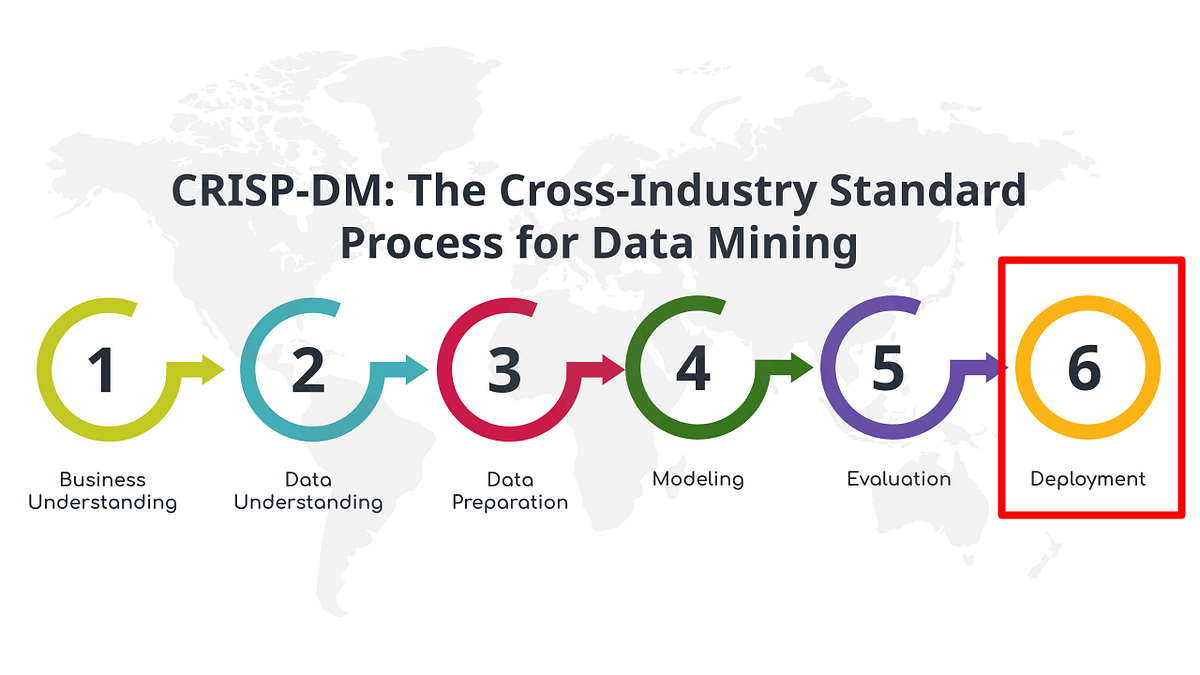
\includegraphics[width=0.9\linewidth]{images/CRISP-DM.png}
\caption{\label{fig:Canasta}La metodología CRISP-DM (Cross Industry Standard Process for Data Mining)}
\end{figure}

\subsection{Pruebas}

\section{Resultados y Conclusiones}


\subsection{How to add Comments and Track Changes}

Comments can be added to your project by highlighting some text and clicking ``Add comment'' in the top right of the editor pane. To view existing comments, click on the Review menu in the toolbar above. To reply to a comment, click on the Reply button in the lower right corner of the comment. You can close the Review pane by clicking its name on the toolbar when you're done reviewing for the time being.

Track changes are available on all our \href{https://www.overleaf.com/user/subscription/plans}{premium plans}, and can be toggled on or off using the option at the top of the Review pane. Track changes allow you to keep track of every change made to the document, along with the person making the change. 

\subsection{How to add Lists}

You can make lists with automatic numbering \dots

\begin{enumerate}
\item Like this,
\item and like this.
\end{enumerate}
\dots or bullet points \dots
\begin{itemize}
\item Like this,
\item and like this.
\end{itemize}

\subsection{How to write Mathematics}

\LaTeX{} is great at typesetting mathematics. Let $X_1, X_2, \ldots, X_n$ be a sequence of independent and identically distributed random variables with $\text{E}[X_i] = \mu$ and $\text{Var}[X_i] = \sigma^2 < \infty$, and let
\[S_n = \frac{X_1 + X_2 + \cdots + X_n}{n}
      = \frac{1}{n}\sum_{i}^{n} X_i\]
denote their mean. Then as $n$ approaches infinity, the random variables $\sqrt{n}(S_n - \mu)$ converge in distribution to a normal $\mathcal{N}(0, \sigma^2)$.


\subsection{How to add Citations and a References List}

\bibliographystyle{alpha}
\bibliography{sample}

\end{document}